\title{2021 年高考数学 全国甲卷-文科}
\date{}
\maketitle

\section*{一、选择题}
本题共12小题，每小题5分，共60分.在每小题给出的四个选项中，只有一项是符合题目要求的.

\begin{question}[points=5]
设集合 $M = \{1,3,5,7,9\}$, $N = \{x \mid 2x > 7\}$, 则 $M \cap N =$ ( )
\begin{choices}
  \item $\{7,9\}$
  \item $\{5,7,9\}$
  \item $\{3,5,7,9\}$
  \item $\{1,3,5,7,9\}$
\end{choices}
\begin{solution}
\textbf{答案：}B

\textbf{分析：}求出集合 $N$ 后可求 $M \cap N$.

\textbf{详解：}$N = \left(\frac{7}{2}, +\infty\right)$, 故 $M \cap N = \{5,7,9\}$.
\end{solution}
\end{question}

\begin{question}[points=5]
为了解某地农村经济情况，对该地农户家庭年收入进行抽样调查，将农户家庭年收入的调查数据整理得到如下频率分布直方图：



根据此频率分布直方图，下面结论中不正确的是（ ）

\begin{center}
  
\includegraphics[width=.38\linewidth]{question-2-1.jpg}
\end{center}
\begin{choices}
  \item A. 该地农户家庭年收入低于4.5万元的农户比率估计为6%
  \item B. 该地农户家庭年收入不低于10.5万元的农户比率估计为10%
  \item C. 估计该地农户家庭年收入的平均值不超过6.5万元
  \item D. 估计该地有一半以上的农户，其家庭年收入介于4.5万元至8.5万元之间
\end{choices}
\begin{solution}
\textbf{答案：}C

\textbf{分析：}根据直方图的意义直接计算相应范围内的频率，即可判定ABD,以各组的中间值作为代表乘以相应的频率，然后求和即得到样本的平均数的估计值，也就是总体平均值的估计值，计算后即可判定C.

\textbf{详解：}因为频率直方图中的组距为1，所以各组的直方图的高度等于频率.样本频率直方图中的频率即可作为总体的相应比率的估计值.

该地农户家庭年收入低于4.5万元的农户的比率估计值为 $0.02+0.04=0.06=6\%$ ,故A正确；
该地农户家庭年收入不低于10.5万元的农户比率估计值为 $0.04+0.02\times3=0.10=10\%$ ,故B正确；
该地农户家庭年收入介于4.5万元至8.5万元之间的比例估计值为 $0.10+0.14+0.20\times2=0.64=64\%>50\%$ ,故D正确；
该地农户家庭年收入的平均值的估计值为 $3\times0.02+4\times0.04+5\times0.10+6\times0.14+7\times0.20+8\times0.20+9\times0.10+10\times0.10+11\times0.04+12\times0.02+13\times0.02+14\times0.02=7.68$ (万元)，超过6.5万元，故C错误.
综上，给出结论中不正确的是C.
\end{solution}
\end{question}

\begin{question}[points=5]
已知 $(1-i)^2 z = 3+2i$, 则 $z =$ ( )
\begin{choices}
  \item $-1-\frac{3}{2}i$
  \item $-1+\frac{3}{2}i$
  \item $-\frac{3}{2}+i$
  \item $-\frac{3}{2}-i$
\end{choices}
\begin{solution}
\textbf{答案：}B

\textbf{分析：}由已知得 $z = \frac{3+2i}{-2i}$, 根据复数除法运算法则，即可求解.

\textbf{详解：}$(1-i)^2 z = -2i z = 3+2i$, $z = \frac{3+2i}{-2i} = \frac{(3+2i)\cdot i}{-2i \cdot i} = \frac{-2+3i}{2} = -1 + \frac{3}{2}i$.
\end{solution}
\end{question}

\begin{question}[points=5]
下列函数中是增函数的为（ ）
\begin{choices}
  \item $f(x) = -x$
  \item $f(x) = \left(\frac{2}{3}\right)^x$
  \item $f(x) = x^2$
  \item $f(x) = \sqrt[3]{x}$
\end{choices}
\begin{solution}
\textbf{答案：}D

\textbf{分析：}根据基本初等函数的性质逐项判断后可得正确的选项.

\textbf{详解：}对于A, $f(x)=-x$ 为 $\mathbb{R}$ 上的减函数，不合题意，舍.
对于B, $f(x)=\left(\frac{2}{3}\right)^x$ 为 $\mathbb{R}$ 上的减函数，不合题意，舍.
对于C, $f(x)=x^2$ 在 $(-\infty,0)$ 为减函数，不合题意，舍.
对于D, $f(x)=\sqrt[3]{x}$ 为 $\mathbb{R}$ 上的增函数，符合题意.
\end{solution}
\end{question}

\begin{question}[points=5]
点 $(3,0)$ 到双曲线 $\frac{x^2}{16} - \frac{y^2}{9} = 1$ 的一条渐近线的距离为（ ）
\begin{choices}
  \item $\frac{9}{5}$
  \item $\frac{8}{5}$
  \item $\frac{6}{5}$
  \item $\frac{4}{5}$
\end{choices}
\begin{solution}
\textbf{答案：}A

\textbf{分析：}首先确定渐近线方程，然后利用点到直线距离公式求得点到一条渐近线的距离即可.

\textbf{详解：}由题意可知，双曲线的渐近线方程为：$\frac{x^2}{16} - \frac{y^2}{9} = 0$, 即 $3x \pm 4y = 0$. 结合对称性，不妨考虑点 $(3,0)$ 到直线 $3x+4y=0$ 的距离：$d = \frac{|9+0|}{\sqrt{9+16}} = \frac{9}{5}$.
\end{solution}
\end{question}

\begin{question}[points=5]
青少年视力是社会普遍关注的问题，视力情况可借助视力表测量．通常用五分记录法和小数记录法记录视力数据，五分记录法的数据 $L$ 和小数记录表的数据 $V$ 的满足 $L = 5 + \lg V$．已知某同学视力的五分记录法的数据为4.9，则其视力的小数记录法的数据为（ ）（$\sqrt[10]{10} \approx 1.259$）
\begin{choices}
  \item 1.5
  \item 1.2
  \item 0.8
  \item 0.6
\end{choices}
\begin{solution}
\textbf{答案：}C

\textbf{分析：}根据 $L,V$ 关系，当 $L=4.9$ 时，求出 $\lg V$, 再用指数表示 $V$, 即可求解.

\textbf{详解：}由 $L=5+\lg V$, 当 $L=4.9$ 时, $\lg V = -0.1$, 则 $V = 10^{-0.1} = 10^{-\frac{1}{10}} = \frac{1}{\sqrt[10]{10}} \approx \frac{1}{1.259} \approx 0.8$.
\end{solution}
\end{question}

\begin{question}[points=5]
在一个正方体中，过顶点 $A$ 的三条棱的中点分别为 $E, F, G$．该正方体截去三棱锥 $A-EFG$ 后，所得多面体的三视图中，正视图如图所示，则相应的侧视图是（ ）

\begin{center}
  
\includegraphics[width=.38\linewidth]{question-7-1.jpg}
\end{center}

\begin{center}
  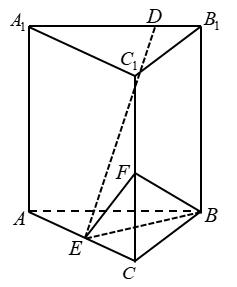
\includegraphics[width=.38\linewidth]{question-7-2.jpg}
\end{center}
\begin{choices}
  \item 
  \item 
  \item 
  \item 
\end{choices}
\begin{solution}
\textbf{答案：}D

\textbf{分析：}根据题意及题目所给的正视图还原出几何体的直观图，结合直观图进行判断.

\textbf{详解：}由题意及正视图可得几何体的直观图，如图所示，

所以其侧视图为

故选：D.
\end{solution}
\end{question}

\begin{question}[points=5]
在 $\triangle ABC$ 中，已知 $B=120^{\circ}$, $AC=\sqrt{19}$, $AB=2$, 则 $BC=$ ( )
\begin{choices}
  \item 1
  \item $\sqrt{2}$
  \item $\sqrt{5}$
  \item 3
\end{choices}
\begin{solution}
\textbf{答案：}D

\textbf{分析：}利用余弦定理得到关于 $BC$ 长度的方程，解方程即可求得边长.

\textbf{详解：}设 $AB=c$, $AC=b$, $BC=a$, 结合余弦定理：$b^2 = a^2 + c^2 - 2ac \cos B$ 可得：$19 = a^2 + 4 - 2 \times a \times \cos 120^{\circ}$, 即 $a^2 + 2a -15 = 0$, 解得 $a=3$（$a=-5$ 舍去），故 $BC=3$.
\end{solution}
\end{question}

\begin{question}[points=5]
记 $S_n$ 为等比数列 $\{a_n\}$ 的前 $n$ 项和.若 $S_2=4$, $S_4=6$, 则 $S_6=$ ( )
\begin{choices}
  \item 7
  \item 8
  \item 9
  \item 10
\end{choices}
\begin{solution}
\textbf{答案：}A

\textbf{分析：}根据题目条件可得 $S_2$, $S_4-S_2$, $S_6-S_4$ 成等比数列，从而求出 $S_6-S_4=1$, 进一步求出答案.

\textbf{详解：}∵ $S_n$ 为等比数列 $\{a_n\}$ 的前 $n$ 项和，∴ $S_2$, $S_4-S_2$, $S_6-S_4$ 成等比数列. ∴ $S_2=4$, $S_4-S_2=6-4=2$, ∴ $S_6-S_4=1$, ∴ $S_6=1+S_4=1+6=7$.
\end{solution}
\end{question}

\begin{question}[points=5]
将3个1和2个0随机排成一行，则2个0不相邻的概率为（ ）
\begin{choices}
  \item 0.3
  \item 0.5
  \item 0.6
  \item 0.8
\end{choices}
\begin{solution}
\textbf{答案：}C

\textbf{分析：}利用古典概型的概率公式可求概率.

\textbf{详解：}将3个1和2个0随机排成一行，共有10种排法：00111,01011,01101,01110,10011,10101,10110,11001,11010,11100. 其中2个0不相邻的排列有6种：01011,01101,01110,10101,10110,11010. 故概率为 $\frac{6}{10}=0.6$.
\end{solution}
\end{question}

\begin{question}[points=5]
若 $\alpha \in \left(0, \frac{\pi}{2}\right)$, $\tan 2\alpha = \frac{\cos \alpha}{2 - \sin \alpha}$, 则 $\tan \alpha =$ ( )
\begin{choices}
  \item $\frac{\sqrt{15}}{15}$
  \item $\frac{\sqrt{5}}{5}$
  \item $\frac{\sqrt{5}}{3}$
  \item $\frac{\sqrt{15}}{3}$
\end{choices}
\begin{solution}
\textbf{答案：}A

\textbf{分析：}由二倍角公式可得 $\tan 2\alpha = \frac{\sin 2\alpha}{\cos 2\alpha} = \frac{2\sin\alpha\cos\alpha}{1-2\sin^2\alpha}$, 再结合已知可求得 $\sin\alpha = \frac{1}{4}$, 利用同角三角函数的基本关系即可求解.

\textbf{详解：}∵ $\tan 2\alpha = \frac{\cos\alpha}{2-\sin\alpha}$, ∴ $\tan 2\alpha = \frac{\sin 2\alpha}{\cos 2\alpha} = \frac{2\sin\alpha\cos\alpha}{1-2\sin^2\alpha} = \frac{\cos\alpha}{2-\sin\alpha}$. ∵ $\alpha \in \left(0, \frac{\pi}{2}\right)$, ∴ $\cos\alpha \neq 0$, ∴ $\frac{2\sin\alpha}{1-2\sin^2\alpha} = \frac{1}{2-\sin\alpha}$, 解得 $\sin\alpha = \frac{1}{4}$. ∴ $\cos\alpha = \sqrt{1-\sin^2\alpha} = \frac{\sqrt{15}}{4}$, ∴ $\tan\alpha = \frac{\sin\alpha}{\cos\alpha} = \frac{\sqrt{15}}{15}$.
\end{solution}
\end{question}

\begin{question}[points=5]
设 $f(x)$ 是定义域为 $\mathbf{R}$ 的奇函数，且 $f(1+x)=f(-x)$. 若 $f\left(-\frac{1}{3}\right) = \frac{1}{3}$, 则 $f\left(\frac{5}{3}\right) =$ ( )
\begin{choices}
  \item $-\frac{5}{3}$
  \item $-\frac{1}{3}$
  \item $\frac{1}{3}$
  \item $\frac{5}{3}$
\end{choices}
\begin{solution}
\textbf{答案：}C

\textbf{分析：}由题意利用函数的奇偶性和函数的递推关系即可求得 $f\left(\frac{5}{3}\right)$ 的值.

\textbf{详解：}$f\left(\frac{5}{3}\right) = f\left(1+\frac{2}{3}\right) = f\left(-\frac{2}{3}\right) = -f\left(\frac{2}{3}\right)$. 而 $f\left(\frac{2}{3}\right) = f\left(1-\frac{1}{3}\right) = f\left(\frac{1}{3}\right) = -f\left(-\frac{1}{3}\right) = -\frac{1}{3}$, 故 $f\left(\frac{5}{3}\right) = \frac{1}{3}$.
\end{solution}
\end{question}

\section*{二、填空题}
本题共4小题，每小题5分，共20分.

\begin{question}[points=5]
若向量 $\vec{a}, \vec{b}$ 满足 $|\vec{a}|=3$, $|\vec{a}-\vec{b}|=5$, $\vec{a}\cdot\vec{b}=1$, 则 $|\vec{b}|=$ .
\fillin[{$3\sqrt{2}$}]
\begin{solution}
\textbf{答案：}$3\sqrt{2}$

\textbf{分析：}根据题目条件，利用 $|\vec{a}-\vec{b}|$ 模的平方可以得出答案.

\textbf{详解：}∵ $|\vec{a}-\vec{b}|=5$, ∴ $|\vec{a}-\vec{b}|^2 = |\vec{a}|^2 + |\vec{b}|^2 - 2\vec{a}\cdot\vec{b} = 9 + |\vec{b}|^2 - 2 = 25$, ∴ $|\vec{b}|^2 = 18$, $|\vec{b}| = 3\sqrt{2}$.
\end{solution}
\end{question}

\begin{question}[points=5]
已知一个圆锥的底面半径为6，其体积为 $30\pi$ 则该圆锥的侧面积为.
\fillin[{$39\pi$}]
\begin{solution}
\textbf{答案：}$39\pi$

\textbf{分析：}利用体积公式求出圆锥的高，进一步求出母线长，最终利用侧面积公式求出答案.

\textbf{详解：}∵ $V = \frac{1}{3}\pi \cdot 6^2 \cdot h = 30\pi$, ∴ $h = \frac{5}{2}$. ∴ $l = \sqrt{h^2 + r^2} = \sqrt{\left(\frac{5}{2}\right)^2 + 6^2} = \frac{13}{2}$. ∴ $S_{\text{侧}} = \pi r l = \pi \times 6 \times \frac{13}{2} = 39\pi$.
\end{solution}
\end{question}

\begin{question}[points=5]
已知函数 $f(x) = 2\cos(\omega x + \varphi)$ 的部分图像如图所示，则 $f\left(\frac{\pi}{2}\right) =$ .

\begin{center}
  
\includegraphics[width=.38\linewidth]{question-15-1.jpg}
\end{center}
\fillin[{$-\sqrt{3}$}]
\begin{solution}
\textbf{答案：}$-\sqrt{3}$

\textbf{分析：}首先确定函数的解析式，然后求解 $f\left(\frac{\pi}{2}\right)$ 的值即可.

\textbf{详解：}由题意可得：$\frac{3}{4}T = \frac{13\pi}{12} - \frac{\pi}{3} = \frac{3\pi}{4}$, ∴ $T = \pi$, $\omega = \frac{2\pi}{T} = 2$. 当 $x = \frac{13\pi}{12}$ 时，$\omega x + \varphi = 2 \times \frac{13\pi}{12} + \varphi = 2k\pi$, ∴ $\varphi = 2k\pi - \frac{13\pi}{6}$ ($k \in \mathbf{Z}$). 令 $k=1$ 可得：$\varphi = -\frac{\pi}{6}$. 据此有：$f(x) = 2\cos\left(2x - \frac{\pi}{6}\right)$, $f\left(\frac{\pi}{2}\right) = 2\cos\left(2\times\frac{\pi}{2} - \frac{\pi}{6}\right) = 2\cos\frac{5\pi}{6} = -\sqrt{3}$.
\end{solution}
\end{question}

\begin{question}[points=5]
已知 $F_1, F_2$ 为椭圆 $C: \frac{x^2}{16} + \frac{y^2}{4} = 1$ 的两个焦点，$P, Q$ 为 $C$ 上关于坐标原点对称的两点，且 $|PQ| = |F_1F_2|$, 则四边形 $PF_1QF_2$ 的面积为.
\fillin[{$8$}]
\begin{solution}
\textbf{答案：}$8$

\textbf{分析：}根据已知可得 $PF_1 \perp PF_2$, 设 $|PF_1| = m$, $|PF_2| = n$, 利用勾股定理结合 $m+n=8$, 求出 $mn$, 四边形 $PF_1QF_2$ 面积等于 $mn$.

\textbf{详解：}因为 $P, Q$ 为 $C$ 上关于坐标原点对称的两点，且 $|PQ| = |F_1F_2|$, 所以四边形 $PF_1QF_2$ 为矩形. 设 $|PF_1| = m$, $|PF_2| = n$, 则 $m+n=8$, $m^2+n^2=48$, 所以 $64 = (m+n)^2 = m^2 + 2mn + n^2 = 48 + 2mn$, 解得 $mn=8$, 即四边形 $PF_1QF_2$ 面积等于 $8$.
\end{solution}
\end{question}

\section*{三、解答题}
共70分.解答应写出文字说明、证明过程或演算步骤.第17~21题为必考题，每个试题考生都必须作答.第22、23题为选考题，考生根据要求作答.

\begin{question}[points=12]
甲、乙两台机床生产同种产品，产品按质量分为一级品和二级品，为了比较两台机床产品的质量，分别用两台机床各生产了200件产品，产品的质量情况统计如下表：



|        | 一级品 | 二级品 | 合计 |

|--------|--------|--------|------|

| 甲机床 | 150    | 50     | 200  |

| 乙机床 | 120    | 80     | 200  |

| 合计   | 270    | 130    | 400  |



（1）甲机床、乙机床生产的产品中一级品的频率分别是多少?



（2）能否有99%的把握认为甲机床的产品质量与乙机床的产品质量有差异?



附：$K^2 = \frac{n(ad-bc)^2}{(a+b)(c+d)(a+c)(b+d)}$



$P(K^2 \ge k)$  0.050  0.010  0.001



$k$          3.841  6.635  10.828
\begin{solution}
\textbf{答案：}（1）75%；60%；（2）能.

\textbf{分析：}根据给出公式计算即可.

\textbf{详解：}（1）甲机床生产的产品中的一级品的频率为 $\frac{150}{200}=75\%$, 乙机床生产的产品中的一级品的频率为 $\frac{120}{200}=60\%$.

（2）$K^2 = \frac{400 \times (150\times80 - 120\times50)^2}{270\times130\times200\times200} = \frac{400}{39} \approx 10.256 > 6.635$, 故能有99%的把握认为甲机床的产品与乙机床的产品质量有差异.
\end{solution}
\end{question}

\begin{question}[points=12]
记 $S_n$ 为数列 $\{a_n\}$ 的前 $n$ 项和，已知 $a_n > 0$, $a_2 = 3a_1$, 且数列 $\{\sqrt{S_n}\}$ 是等差数列，证明：$\{a_n\}$ 是等差数列.
\begin{solution}
\textbf{答案：}证明见解析.

\textbf{分析：}先根据 $\sqrt{S_2} - \sqrt{S_1}$ 求出数列 $\{\sqrt{S_n}\}$ 的公差 $d$, 进一步写出 $\{\sqrt{S_n}\}$ 的通项，从而求出 $\{a_n\}$ 的通项公式，最终得证.

\textbf{详解：}∵数列 $\{\sqrt{S_n}\}$ 是等差数列，设公差为 $d = \sqrt{S_2} - \sqrt{S_1} = \sqrt{a_2} - \sqrt{a_1} = \sqrt{3a_1} - \sqrt{a_1} = \sqrt{a_1}(\sqrt{3}-1)$. 由 $a_2=3a_1$ 得 $d=\sqrt{a_1}(\sqrt{3}-1)$. 又 $\sqrt{S_1}=\sqrt{a_1}$, 所以 $\sqrt{S_n} = \sqrt{a_1} + (n-1)d = \sqrt{a_1} + (n-1)\sqrt{a_1}(\sqrt{3}-1) = \sqrt{a_1}((\sqrt{3}-1)n + 2-\sqrt{3})$. 则 $S_n = a_1[((\sqrt{3}-1)n + 2-\sqrt{3})^2]$. 当 $n\ge 2$ 时, $a_n = S_n - S_{n-1} = a_1[((\sqrt{3}-1)n + 2-\sqrt{3})^2 - ((\sqrt{3}-1)(n-1) + 2-\sqrt{3})^2] = a_1[2(\sqrt{3}-1)^2 n + 2(\sqrt{3}-1)(2-\sqrt{3}) - (\sqrt{3}-1)^2]$. 整理得 $a_n = 2a_1(\sqrt{3}-1)^2 n + a_1[2(\sqrt{3}-1)(2-\sqrt{3}) - (\sqrt{3}-1)^2]$. 计算可知 $a_n - a_{n-1} = 2a_1(\sqrt{3}-1)^2$ 为常数，故 $\{a_n\}$ 是等差数列.
\end{solution}
\end{question}

\begin{question}[points=12]
已知直三棱柱 $ABC-A_1B_1C_1$ 中，侧面 $AA_1B_1B$ 为正方形，$AB=BC=2$, $E, F$ 分别为 $AC$ 和 $CC_1$ 的中点，$BF \perp A_1B_1$.



（1）求三棱锥 $F-EBC$ 的体积；



（2）已知 $D$ 为棱 $A_1B_1$ 上的点，证明：$BF \perp DE$.
\begin{solution}
\textbf{答案：}(1) $\frac{1}{3}$；(2)证明见解析.

\textbf{分析：}(1)首先求得 $AC$ 的长度，然后利用体积公式可得三棱锥的体积；(2)将所给的几何体进行补形，从而把线线垂直的问题转化为证明线面垂直，然后再由线面垂直可得题中的结论.

\textbf{详解：}(1)如图所示，连结 $AF$. 由题意可得：$BF = \sqrt{BC^2 + CF^2} = \sqrt{4+1} = \sqrt{5}$. 由于 $AB \perp BB_1$, $BC \perp AB$, $BB_1 \cap BC = B$, 故 $AB \perp$ 平面 $BCC_1B_1$, 而 $BF \subset$ 平面 $BCC_1B_1$, 故 $AB \perp BF$, 从而有 $AF = \sqrt{AB^2 + BF^2} = \sqrt{4+5} = 3$, 从而 $AC = \sqrt{AF^2 - CF^2} = \sqrt{9-1} = 2\sqrt{2}$, 则 $AB^2 + BC^2 = AC^2$, ∴ $AB \perp BC$, $\triangle ABC$ 为等腰直角三角形. $S_{\triangle BCE} = \frac{1}{2} S_{\triangle ABC} = \frac{1}{2} \times \frac{1}{2} \times 2 \times 2 = 1$, $V_{F-EBC} = \frac{1}{3} S_{\triangle BCE} \times CF = \frac{1}{3} \times 1 \times 1 = \frac{1}{3}$.

(2)由(1)的结论可将几何体补形为一个棱长为2的正方体 $ABCM-A_1B_1C_1M_1$, 如图所示，取棱 $AM, BC$ 的中点 $H, G$, 连结 $A_1H, HG, GB_1$. 正方形 $BCC_1B_1$ 中, $G, F$ 为中点, 则 $BF \perp B_1G$, 又 $BF \perp A_1B_1$, $A_1B_1 \cap B_1G = B_1$, 故 $BF \perp$ 平面 $A_1B_1GH$, 而 $DE \subset$ 平面 $A_1B_1GH$, 从而 $BF \perp DE$.
\end{solution}
\end{question}

\begin{question}[points=12]
设函数 $f(x) = a^2 x^2 + ax - 3\ln x + 1$, 其中 $a>0$.



（1）讨论 $f(x)$ 的单调性；



（2）若 $y=f(x)$ 的图象与 $x$ 轴没有公共点，求 $a$ 的取值范围.
\begin{solution}
\textbf{答案：}（1）$f(x)$ 的减区间为 $\left(0, \frac{1}{a}\right)$, 增区间为 $\left(\frac{1}{a}, +\infty\right)$；（2）$a > \frac{1}{e}$.

\textbf{分析：}（1）求出函数的导数，讨论其符号后可得函数的单调性.（2）根据 $f(1)>0$ 及（1）的单调性性可得 $f(x)_{\min} > 0$, 从而可求 $a$ 的取值范围.

\textbf{详解：}（1）函数的定义域为 $(0, +\infty)$, 又 $f'(x) = \frac{(2ax+3)(ax-1)}{x}$. 因为 $a>0$, $x>0$, 故 $2ax+3>0$. 当 $0 < x < \frac{1}{a}$ 时, $f'(x) < 0$; 当 $x > \frac{1}{a}$ 时, $f'(x) > 0$. 所以 $f(x)$ 的减区间为 $\left(0, \frac{1}{a}\right)$, 增区间为 $\left(\frac{1}{a}, +\infty\right)$.

（2）因为 $f(1)=a^2+a+1>0$ 且 $y=f(x)$ 的图与 $x$ 轴没有公共点, 所以 $y=f(x)$ 的图象在 $x$ 轴的上方. 由（1）中函数的单调性可得 $f(x)_{\min} = f\left(\frac{1}{a}\right) = 3 - 3\ln\frac{1}{a} = 3 + 3\ln a$, 故 $3+3\ln a > 0$ 即 $a > \frac{1}{e}$.
\end{solution}
\end{question}

\begin{question}[points=12]
抛物线 $C$ 的顶点为坐标原点 $O$．焦点在 $x$ 轴上，直线 $l: x=1$ 交 $C$ 于 $P, Q$ 两点，且 $OP \perp OQ$．已知点 $M(2,0)$, 且 $\bigodot M$ 与 $l$ 相切．



（1）求 $C$, $\bigodot M$ 的方程；



（2）设 $A_1, A_2, A_3$ 是 $C$ 上的三个点，直线 $A_1A_2$, $A_1A_3$ 均与 $\bigodot M$ 相切．判断直线 $A_2A_3$ 与 $\bigodot M$ 的位置关系，并说明理由．
\begin{solution}
\textbf{答案：}（1）抛物线 $C: y^2 = x$, $\bigodot M$ 方程为 $(x-2)^2 + y^2 = 1$；（2）相切，理由见解析.

\textbf{分析：}（1）根据已知抛物线与 $x=1$ 相交，可得出抛物线开口向右，设出标准方程，再利用对称性设出 $P, Q$ 坐标，由 $OP \perp OQ$, 即可求出 $p$；由圆 $M$ 与直线 $x=1$ 相切，求出半径，即可得出结论；（2）先考虑 $A_1A_2$ 斜率不存在情况，根据对称性，即可得出结论；若 $A_1A_2, A_1A_3, A_2A_3$ 斜率存在，由 $A_1, A_2, A_3$ 三点在抛物线上，将直线 $A_1A_2$, $A_1A_3$, $A_2A_3$ 斜率分别用纵坐标表示，再由 $A_1A_2$, $A_1A_3$ 与圆 $M$ 相切，得出 $y_2+y_3$, $y_2y_3$ 与 $y_1$ 的关系，最后求出 $M$ 点到直线 $A_2A_3$ 的距离，即可得出结论.

\textbf{详解：}（1）依题意设抛物线 $C: y^2 = 2px (p>0)$, $P(1, y_0)$, $Q(1, -y_0)$. ∵ $OP \perp OQ$, ∴ $\overrightarrow{OP} \cdot \overrightarrow{OQ} = 1 - y_0^2 = 1 - 2p = 0$, ∴ $2p=1$, 所以抛物线 $C$ 的方程为 $y^2 = x$. $M(2,0)$, $\bigodot M$ 与 $x=1$ 相切，所以半径为 $1$, 所以 $\bigodot M$ 的方程为 $(x-2)^2 + y^2 = 1$.

（2）设 $A_1(x_1, y_1)$, $A_2(x_2, y_2)$, $A_3(x_3, y_3)$. 若 $A_1A_2$ 斜率不存在，则 $A_1A_2$ 方程为 $x=1$ 或 $x=3$. 若 $A_1A_2$ 方程为 $x=1$, 根据对称性不妨设 $A_1(1,1)$, 则过 $A_1$ 与圆 $M$ 相切的另一条直线方程为 $y=1$, 此时该直线与抛物线只有一个交点，即不存在 $A_3$, 不合题意. 若 $A_1A_2$ 方程为 $x=3$, 根据对称性不妨设 $A_1(3,\sqrt{3})$, $A_2(3,-\sqrt{3})$, 则过 $A_1$ 与圆 $M$ 相切的直线 $A_1A_3$ 为 $y-\sqrt{3} = \frac{\sqrt{3}}{3}(x-3)$, 又 $k_{A_1A_3} = \frac{1}{y_1+y_3} = \frac{1}{\sqrt{3}+y_3} = \frac{\sqrt{3}}{3}$, ∴ $y_3=0$, $x_3=0$, $A_3(0,0)$, 此时直线 $A_1A_3$, $A_2A_3$ 关于 $x$ 轴对称，所以直线 $A_2A_3$ 与圆 $M$ 相切.

若直线 $A_1A_2$, $A_1A_3$, $A_2A_3$ 斜率均存在，则 $k_{A_1A_2} = \frac{1}{y_1+y_2}$, $k_{A_1A_3} = \frac{1}{y_1+y_3}$, $k_{A_2A_3} = \frac{1}{y_2+y_3}$. 所以直线 $A_1A_2$ 方程为 $x - (y_1+y_2)y + y_1y_2 = 0$, 同理直线 $A_1A_3$ 方程为 $x - (y_1+y_3)y + y_1y_3 = 0$, 直线 $A_2A_3$ 方程为 $x - (y_2+y_3)y + y_2y_3 = 0$. ∵ $A_1A_2$ 与圆 $M$ 相切, ∴ $\frac{|2 + y_1y_2|}{\sqrt{1+(y_1+y_2)^2}} = 1$, 整理得 $(y_1^2-1)y_2^2 + 2y_1y_2 + 3 - y_1^2 = 0$. 同理 $(y_1^2-1)y_3^2 + 2y_1y_3 + 3 - y_1^2 = 0$. 所以 $y_2, y_3$ 为方程 $(y_1^2-1)y^2 + 2y_1y + 3 - y_1^2 = 0$ 的两根, ∴ $y_2+y_3 = -\frac{2y_1}{y_1^2-1}$, $y_2y_3 = \frac{3 - y_1^2}{y_1^2-1}$. $M$ 到直线 $A_2A_3$ 的距离为 $d = \frac{|2 + y_2y_3|}{\sqrt{1+(y_2+y_3)^2}} = \frac{|2 + \frac{3-y_1^2}{y_1^2-1}|}{\sqrt{1+\left(-\frac{2y_1}{y_1^2-1}\right)^2}} = \frac{|\frac{y_1^2+1}{y_1^2-1}|}{\sqrt{\frac{(y_1^2-1)^2+4y_1^2}{(y_1^2-1)^2}}} = \frac{y_1^2+1}{\sqrt{(y_1^2+1)^2}} = 1$. 所以直线 $A_2A_3$ 与圆 $M$ 相切.

综上，若直线 $A_1A_2$, $A_1A_3$ 与圆 $M$ 相切，则直线 $A_2A_3$ 与圆 $M$ 相切.
\end{solution}
\end{question}

\section*{四、选考题}
共10分.请考生在第22、23题中任选一题作答.如果多做，则按所做的第一题计分.

\begin{question}[points=10]
[选修4-4：坐标系与参数方程]



在直角坐标系 $xOy$ 中，以坐标原点为极点，$x$ 轴正半轴为极轴建立极坐标系，曲线 $C$ 的极坐标方程为 $\rho = 2\sqrt{2}\cos\theta$.



（1）将 $C$ 的极坐标方程化为直角坐标方程；



（2）设点 $A$ 的直角坐标为 $(1,0)$, $M$ 为 $C$ 上的动点，点 $P$ 满足 $\overrightarrow{AP} = \sqrt{2}\overrightarrow{AM}$, 写出 $P$ 的轨迹 $C_1$ 的参数方程，并判断 $C$ 与 $C_1$ 是否有公共点．
\begin{solution}
\textbf{答案：}（1）$(x-\sqrt{2})^2 + y^2 = 2$；（2）$P$ 的轨迹 $C_1$ 的参数方程为 $\begin{cases} x = 3 - \sqrt{2} + \sqrt{2}\cos\theta \\ y = \sqrt{2}\sin\theta \end{cases}$ ($\theta$ 为参数)，$C$ 与 $C_1$ 没有公共点.

\textbf{分析：}（1）将曲线 $C$ 的极坐标方程化为 $\rho^2 = 2\sqrt{2}\rho\cos\theta$, 将 $x=\rho\cos\theta$, $y=\rho\sin\theta$ 代入可得；（2）设 $P(x,y)$, 设 $M(\sqrt{2}+\sqrt{2}\cos\theta, \sqrt{2}\sin\theta)$, 根据向量关系即可求得 $P$ 的轨迹 $C_1$ 的参数方程，求出两圆圆心距，和半径之差比较可得.

\textbf{详解：}（1）由曲线 $C$ 的极坐标方程 $\rho = 2\sqrt{2}\cos\theta$ 可得 $\rho^2 = 2\sqrt{2}\rho\cos\theta$, 将 $x=\rho\cos\theta$, $y=\rho\sin\theta$ 代入可得 $x^2+y^2 = 2\sqrt{2}x$, 即 $(x-\sqrt{2})^2 + y^2 = 2$.

（2）设 $P(x,y)$, 设 $M(\sqrt{2}+\sqrt{2}\cos\theta, \sqrt{2}\sin\theta)$. ∵ $\overrightarrow{AP} = \sqrt{2}\overrightarrow{AM}$, ∴ $(x-1, y) = \sqrt{2}(\sqrt{2}+\sqrt{2}\cos\theta - 1, \sqrt{2}\sin\theta) = (2+2\cos\theta - \sqrt{2}, 2\sin\theta)$. 则 $\begin{cases} x-1 = 2+2\cos\theta - \sqrt{2} \\ y = 2\sin\theta \end{cases}$, 即 $\begin{cases} x = 3 - \sqrt{2} + 2\cos\theta \\ y = 2\sin\theta \end{cases}$. 故 $P$ 的轨迹 $C_1$ 的参数方程为 $\begin{cases} x = 3 - \sqrt{2} + 2\cos\theta \\ y = 2\sin\theta \end{cases}$ ($\theta$ 为参数). 曲线 $C$ 的圆心为 $(\sqrt{2},0)$, 半径为 $\sqrt{2}$, 曲线 $C_1$ 的圆心为 $(3-\sqrt{2},0)$, 半径为 $2$, 则圆心距为 $3-2\sqrt{2}$, ∵ $3-2\sqrt{2} < 2 - \sqrt{2}$, ∴ 两圆内含, 故曲线 $C$ 与 $C_1$ 没有公共点.
\end{solution}
\end{question}

\begin{question}[points=10]
[选修4-5：不等式选讲]



已知函数 $f(x) = |x-2|$, $g(x) = |2x+3| - |2x-1|$.



（1）画出 $y=f(x)$ 和 $y=g(x)$ 的图像；



（2）若 $f(x+a) \ge g(x)$, 求 $a$ 的取值范围．

\begin{center}
  
\includegraphics[width=.38\linewidth]{question-23-1.jpg}
\end{center}
\begin{solution}
\textbf{答案：}（1）图像见解析；（2）$a \ge \frac{11}{2}$.

\textbf{分析：}（1）分段去绝对值即可画出图像；（2）根据函数图像数形结合可得需将 $y=f(x)$ 向左平移可满足条件，求得 $y=f(x+a)$ 过 $A\left(\frac{1}{2},4\right)$ 时 $a$ 的值可求.

\textbf{详解：}（1）$f(x) = |x-2| = \begin{cases} 2-x, & x<2 \\ x-2, & x\ge 2 \end{cases}$, 画出图像如下：

$g(x) = |2x+3| - |2x-1| = \begin{cases} -4, & x<-\frac{3}{2} \\ 4x+2, & -\frac{3}{2} \le x < \frac{1}{2} \\ 4, & x\ge \frac{1}{2} \end{cases}$, 画出函数图像如下：

（2）$f(x+a) = |x+a-2|$, 如图，在同一个坐标系里画出 $f(x)$, $g(x)$ 图像, $y=f(x+a)$ 是 $y=f(x)$ 平移了 $a$ 个单位得到，则要使 $f(x+a) \ge g(x)$, 需将 $y=f(x)$ 向左平移，即 $a>0$. 当 $y=f(x+a)$ 过 $A\left(\frac{1}{2},4\right)$ 时, $|\frac{1}{2}+a-2| = 4$, 解得 $a = \frac{11}{2}$ 或 $a = -\frac{5}{2}$（舍去）. 则数形结合可得需至少将 $y=f(x)$ 向左平移 $\frac{11}{2}$ 个单位, ∴ $a \ge \frac{11}{2}$.
\end{solution}
\end{question}

